\newpage


\section{Requirements Engineering}\label{sec:requirements-engineering}

\subsection{Requirement Document}\label{subsec:requirement-document}

The document is structured to facilitate the collection of requirements from stakeholders in a clear and systematic
manner. At its core, the document consists of a table where stakeholders are required to fill out specific fields
related to the system requirements. The table is designed to capture both functional and non-functional requirements,
providing the foundation for further analysis and prioritization by the \ac{PO}. The empty template that was circulated
to stakeholders for completion can also be found in \ref{sec:requirement-document} of the paper, providing a
reference for how the requirements were initially collected.

\begin{table}[H]
    \centering
    \footnotesize
    \resizebox{\textwidth}{!}{  % Skaliert die Tabelle auf die Seitenbreite.
        \begin{tabular}{|p{3cm}|p{5cm}|p{4cm}|p{3cm}|p{2cm}|p{2cm}|p{3cm}|p{2.5cm}|}
            \hline
            \textbf{Requirement ID (to be filled by PO)} &
            \textbf{Description (to be filled by Stakeholder)} &
            \textbf{Functional/Non-Functional (to be filled by Stakeholder)} &
            \textbf{Stakeholder (to be filled by Stakeholder)} &
            \textbf{Priority (to be filled by PO)} &
            \textbf{Status (to be filled by PO)} &
            \textbf{Comments/Notes (to be filled by PO)} &
            \textbf{Last Updated (to be filled by PO)} \\ \hline
            & & & & & & & \\ \hline % leere Zeile
            & & & & & & & \\ \hline % leere Zeile
            & & & & & & & \\ \hline % leere Zeile
            & & & & & & & \\ \hline % leere Zeile
            & & & & & & & \\ \hline % leere Zeile
        \end{tabular}
    }
    \caption[Requirement Collection Table]{Requirement Collection Table \footnotemark}
    \label{tab:requirement_collection_table}
\end{table}
\footnotetext{Own illustration}

Each row in the table corresponds to a unique requirement. The first field, the "Requirement ID," is reserved for the
\acs{PO} to assign a unique identifier to each requirement once it has been submitted. This ensures proper traceability
and management of requirements across various phases of the project. Following this, the "Description" field is intended
for stakeholders to provide a detailed explanation of what they expect the system to do. It emphasizes the need for
precision, encouraging stakeholders to specify whether the requirement pertains to a particular system behavior or
performance characteristic.

The table also includes a "Functional/Non-Functional" column, where stakeholders are asked to categorize their
requirement. If the requirement pertains to what the system should do, it is considered functional. Non-functional
requirements, on the other hand, describe how the system performs in terms of attributes such as speed, reliability, or
security. To accommodate any uncertainties, the stakeholders are informed that they can leave this classification to be
determined during subsequent discussions with the \acs{PO}, should they find it difficult to distinguish between the
two.

Another key component is the "Stakeholder" field, where individuals or teams responsible for submitting the requirement
are identified. This enables clear accountability and provides a way to trace the origins of each requirement back to
its respective department or stakeholder.

To ensure that stakeholders understand how to complete their portion of the table, a comprehensive guidance section
follows the table. This guidance elaborates on each field that needs to be filled, providing examples and
clarifications. It emphasizes the importance of clarity in the description, guiding stakeholders to avoid ambiguity, and
includes explanations of both functional and non-functional requirements. Additionally, the guidance outlines how to
identify themselves as stakeholders, ensuring that their input is properly documented.

The remainder of the table, including fields such as "Priority," "Status," "Comments/Notes," and "Last Updated," is
reserved for the \acs{PO} to complete after the requirements have been collected. These fields will be used to
prioritize, track the progress, and document any changes or updates to each requirement, ensuring that the project
remains aligned with both stakeholder expectations and project constraints as it evolves.

This structure ensures a well-organized process for gathering, documenting, and managing system requirements, fostering
collaboration between the stakeholders and the \acs{PO}.

\subsection{Requirement Elicitation}\label{subsec:requirement-elicitation}

During the Requirement Elicitation phase, a combination of structured workshops and ad-hoc meetings via Microsoft Teams
played a central role in defining both the system requirements and the associated business processes. These sessions
provided a platform for stakeholders, domain experts, and the \acs{PO} to collaborate closely, ensuring that the
chatbot’s functionalities would align with the operational needs of the procurement process. Throughout these meetings,
key requirements were identified and discussed in detail, laying the groundwork for the chatbot’s behavior, such as
understanding user needs, searching through supplier catalogs, and facilitating procurement requests. A critical outcome
of these discussions was the definition of core business processes, which were visualized in Miro to provide a clear
understanding of how the chatbot would integrate into existing workflows. One example business process can be found in
figure \ref{fig:DefinedBusinessProcessinMiro}. By mapping out these processes collaboratively, the stakeholder and
\acs{PO} was able to capture the procedural steps the chatbot would follow, ensuring that both functional and
non-functional requirements were well understood and aligned with the organizational objectives.

\begin{figure}[H]
    \centering
    \caption[Defined Business Process in Miro]{Defined Business Process in Miro \footnotemark}
    \label{fig:DefinedBusinessProcessinMiro}
    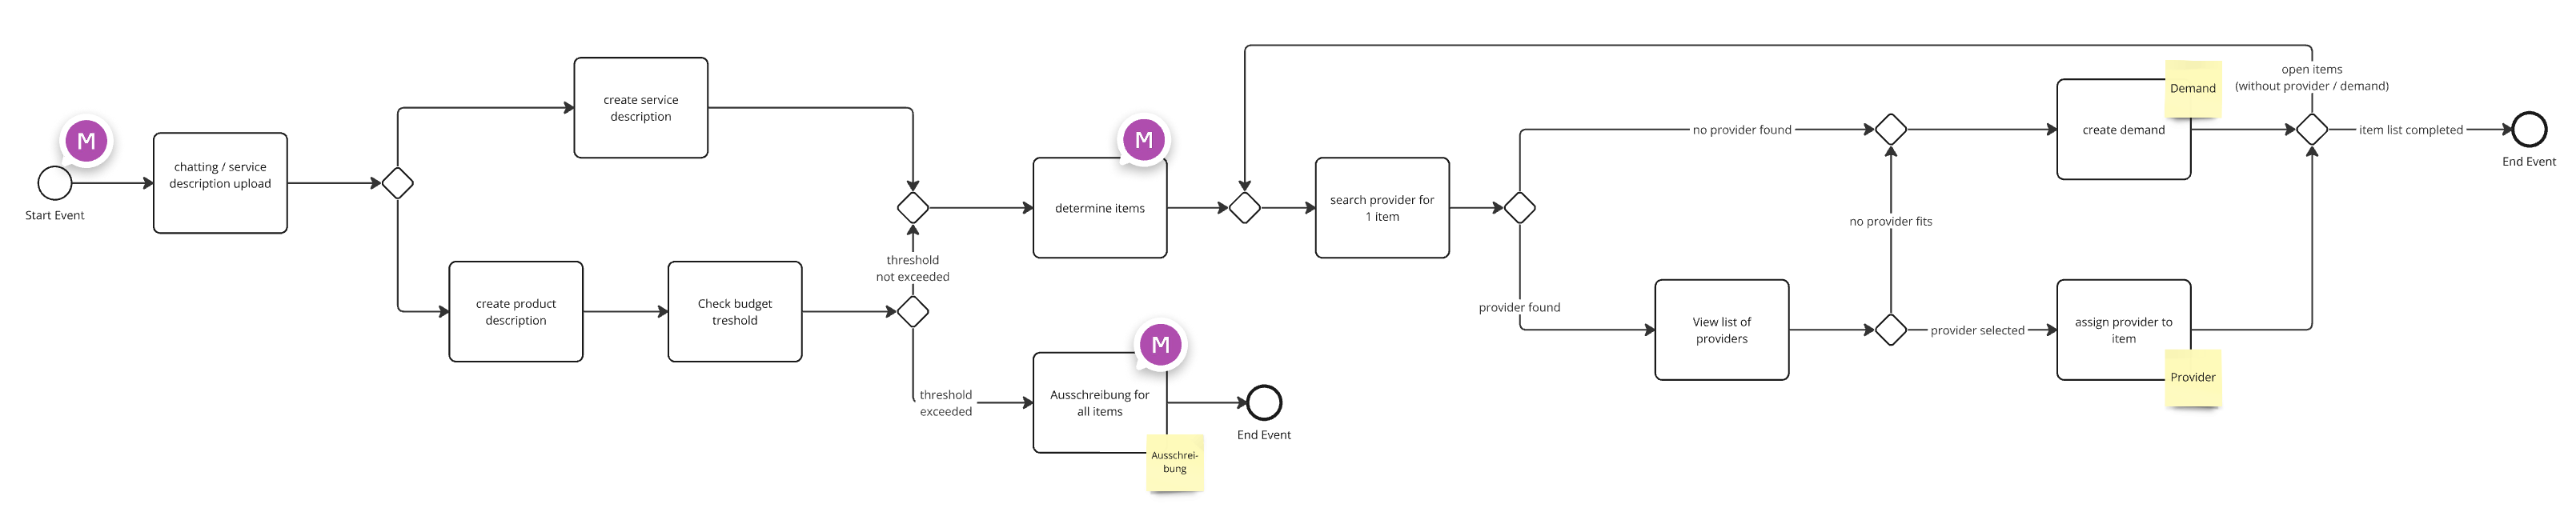
\includegraphics[width=1\textwidth]{abbildungen/RE/Miro/Miro_Business-Process}
\end{figure}
\footnotetext{Own illustration}

As these discussions progressed, certain requirements emerged as more complex or abstract, making them difficult to
fully articulate through conversation alone. In these cases, prototyping became an essential tool for refining and
simplifying these requirements. The Miro mockups, 2 examples shown in figure \ref{fig:ScreenMock-UpsinMiro}, provided an
early-stage visualization of how users would engage with the system, focusing on key interaction points, such as the
user inputting a request, the chatbot interpreting the need, and the subsequent search of supplier catalogs for relevant
offerings. All Miro Screen Mock-Ups can be found in \ref{subsec:screen-mock-ups-in-miro}. These early designs enabled
stakeholders to visualize the flow of operations and provided a concrete foundation for discussions, allowing for
immediate feedback and refinement. The outcome of these discussions clarified the scope of the chatbot's tasks and
helped prioritize functionalities, ensuring that the system would meet the diverse requirements of both end-users and
the internal procurement processes.

\begin{figure}[H]
    \centering
    \caption[Screen Mock-Ups in Miro]{Screen Mock-Ups in Miro \footnotemark}
    \label{fig:ScreenMock-UpsinMiro}
    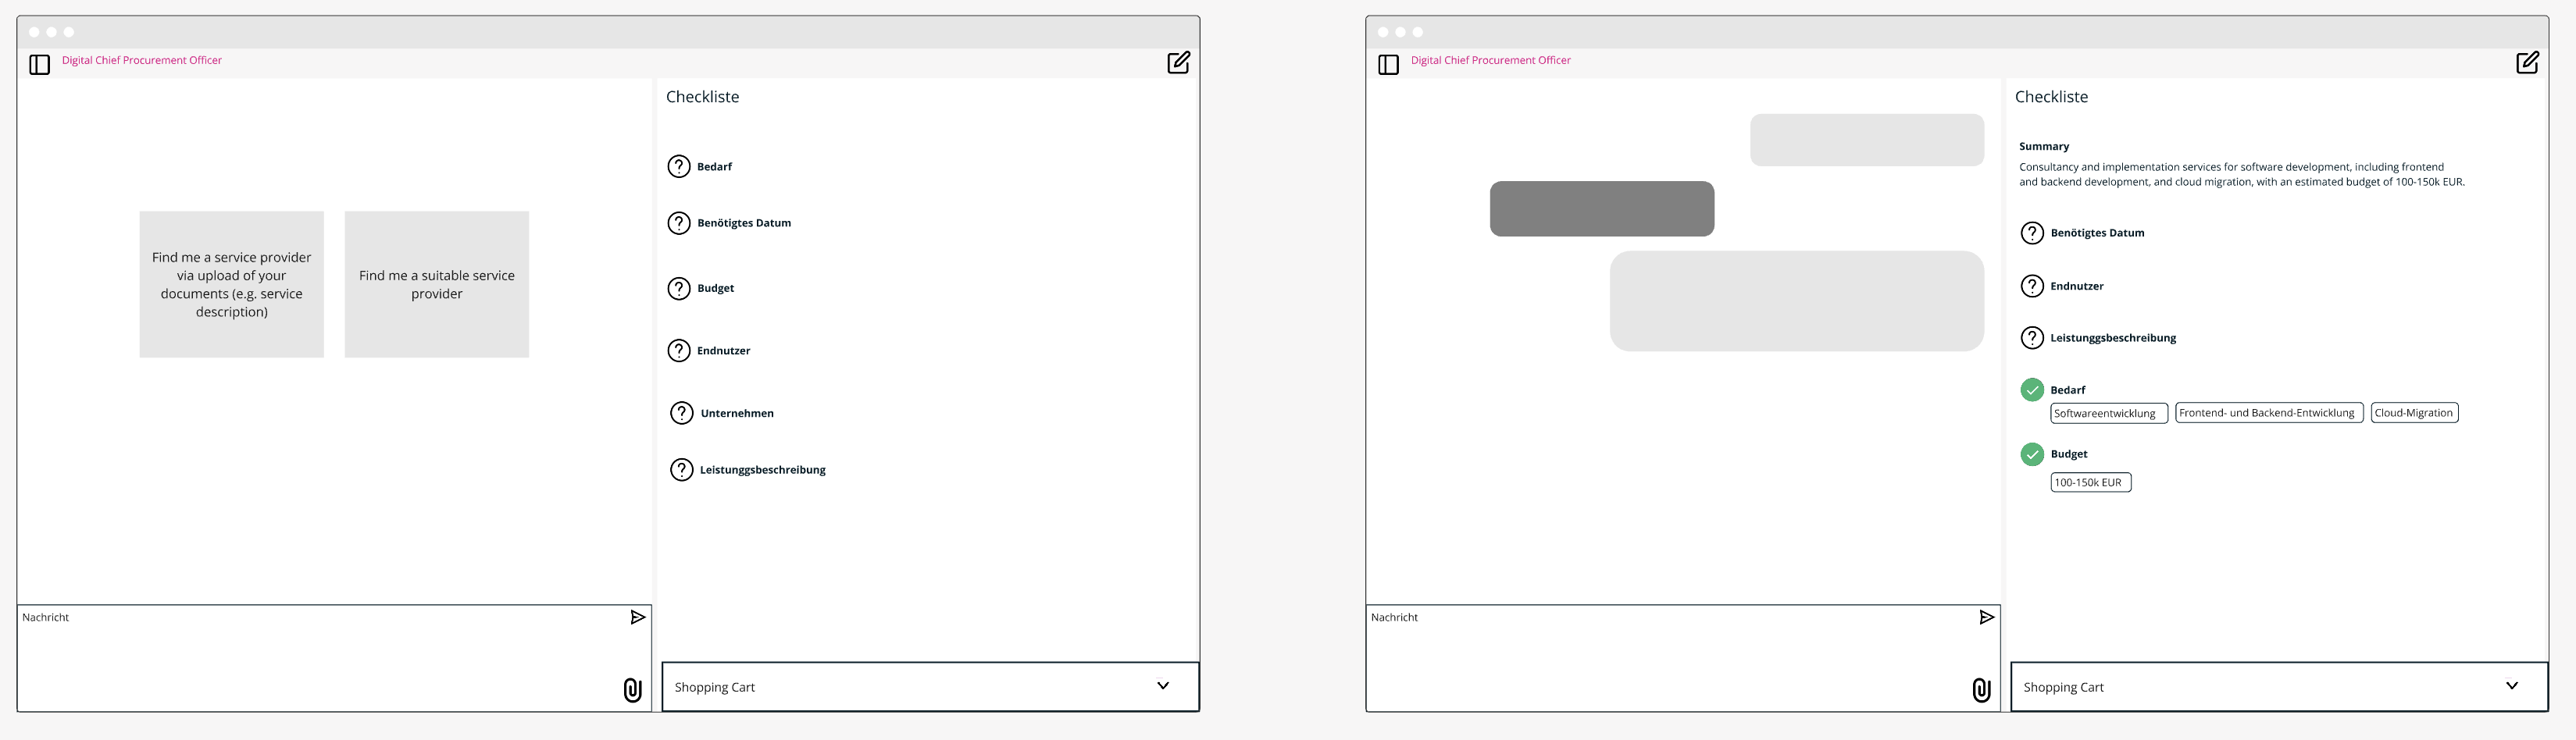
\includegraphics[width=1\textwidth]{abbildungen/RE/Miro/Miro_Mockups}
\end{figure}
\footnotetext{Own illustration}

Building on these initial mockups, the project transitioned to more detailed prototyping in Figma. The initial concepts
developed in Miro were translated into high-fidelity interactive designs, offering a more precise depiction of the user
interface and interaction flows. The Figma prototypes, examples shown in figure \ref{fig:ScreenPrototypeFigmaLM} and
figure \ref{fig:ScreenPrototypeFigmaDM}, allowed stakeholders to experience a more realistic representation
of the chatbot, including how it would handle user queries, present search results from supplier catalogs, and guide the
user through the selection and checkout process. All Figma Screen Prototypes can be found in
\ref{subsec:screen-prototypes-in-figma}. This phase proved critical in refining the system’s requirements, as
the visual and interactive nature of the Figma screens enabled stakeholders to provide targeted feedback on specific
elements of the interface, including the chatbot’s responses, the organization of data, and the overall user experience.
As the designs became more detailed, the stakeholder was able to refine aspects such as response times, data handling,
and catalog integration, ensuring that the chatbot’s functionalities aligned with both the technical capabilities of the
system and the users’ expectations.

\begin{figure}[H]
    \centering
    \caption[Screen Prototype in Figma (Lightmode)]{Screen Prototype in Figma (Lightmode) \footnotemark}
    \label{fig:ScreenPrototypeFigmaLM}
    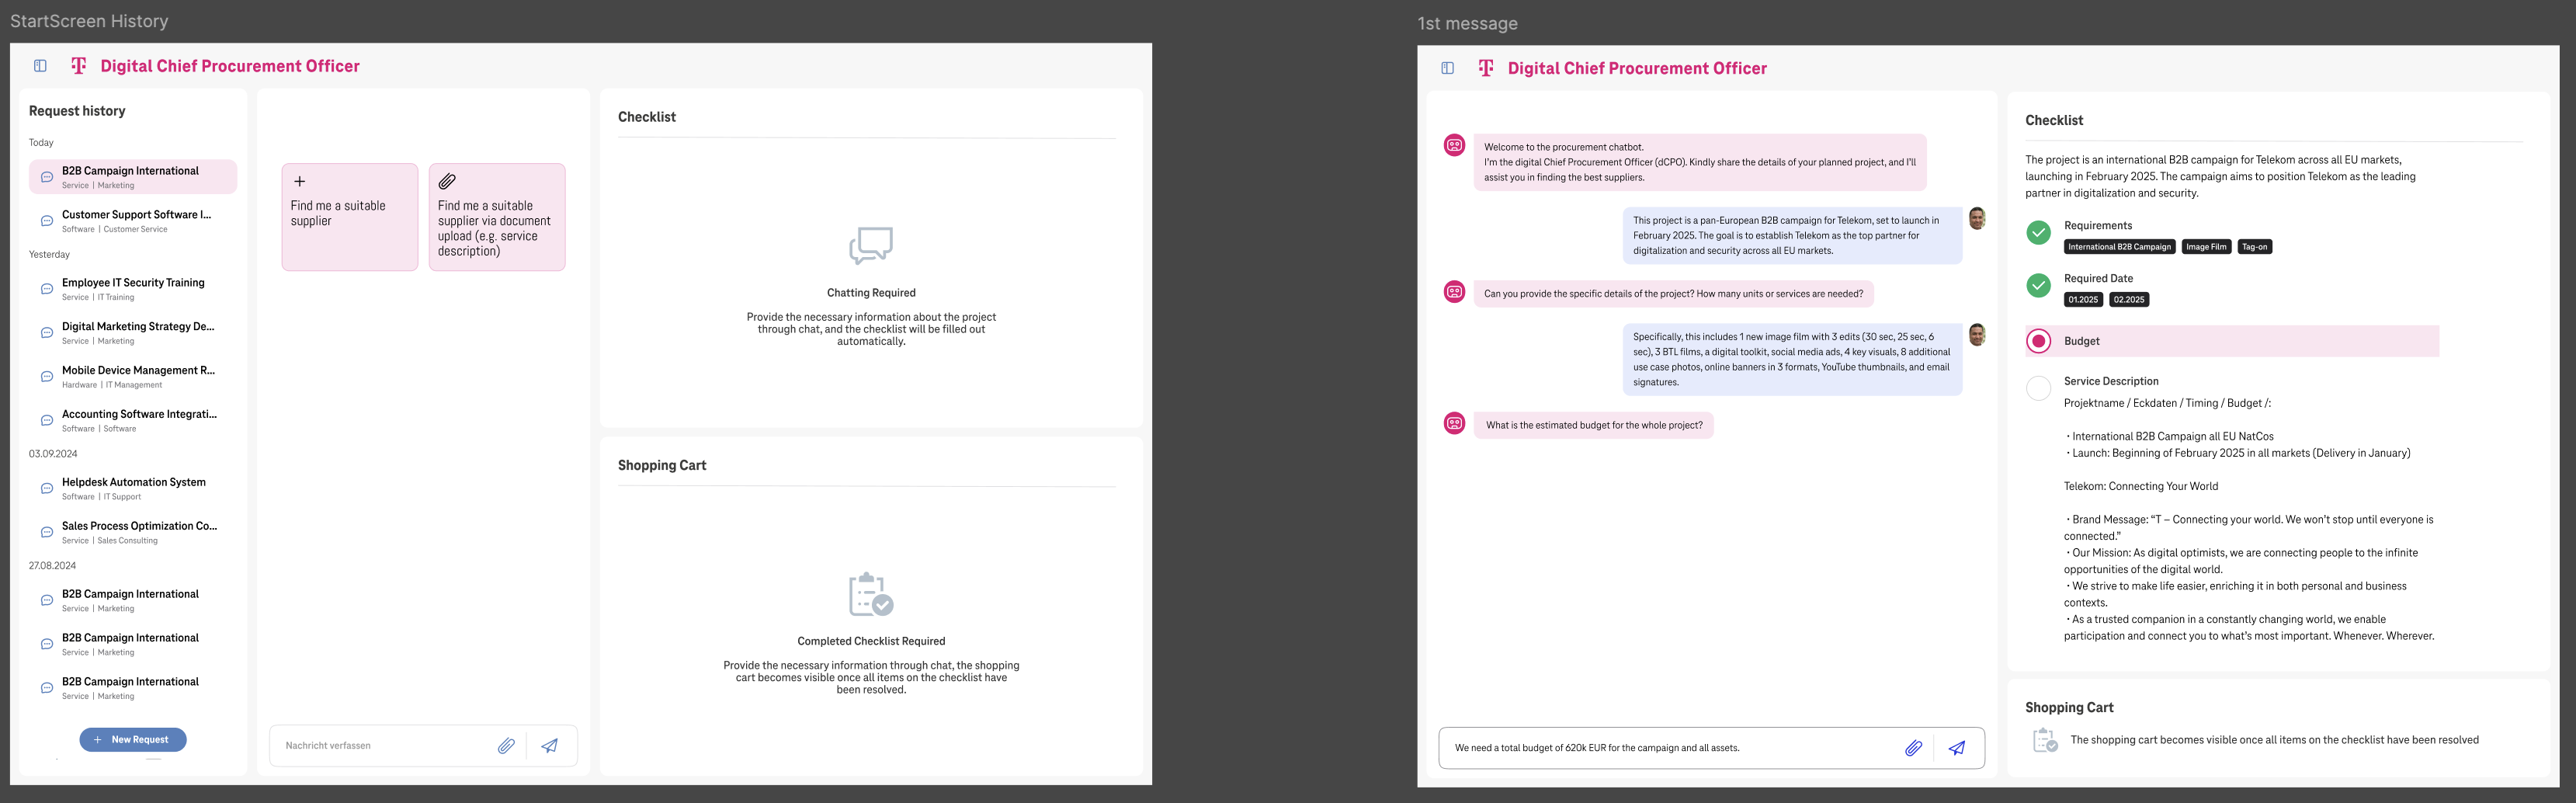
\includegraphics[width=1\textwidth]{abbildungen/RE/Figma/Figma_Screens-Lightmode}
\end{figure}
\footnotetext{Own illustration}

\begin{figure}[H]
    \centering
    \caption[Screen Prototype in Figma (Darkmode)]{Screen Prototype in Figma (Darkmode) \footnotemark}
    \label{fig:ScreenPrototypeFigmaDM}
    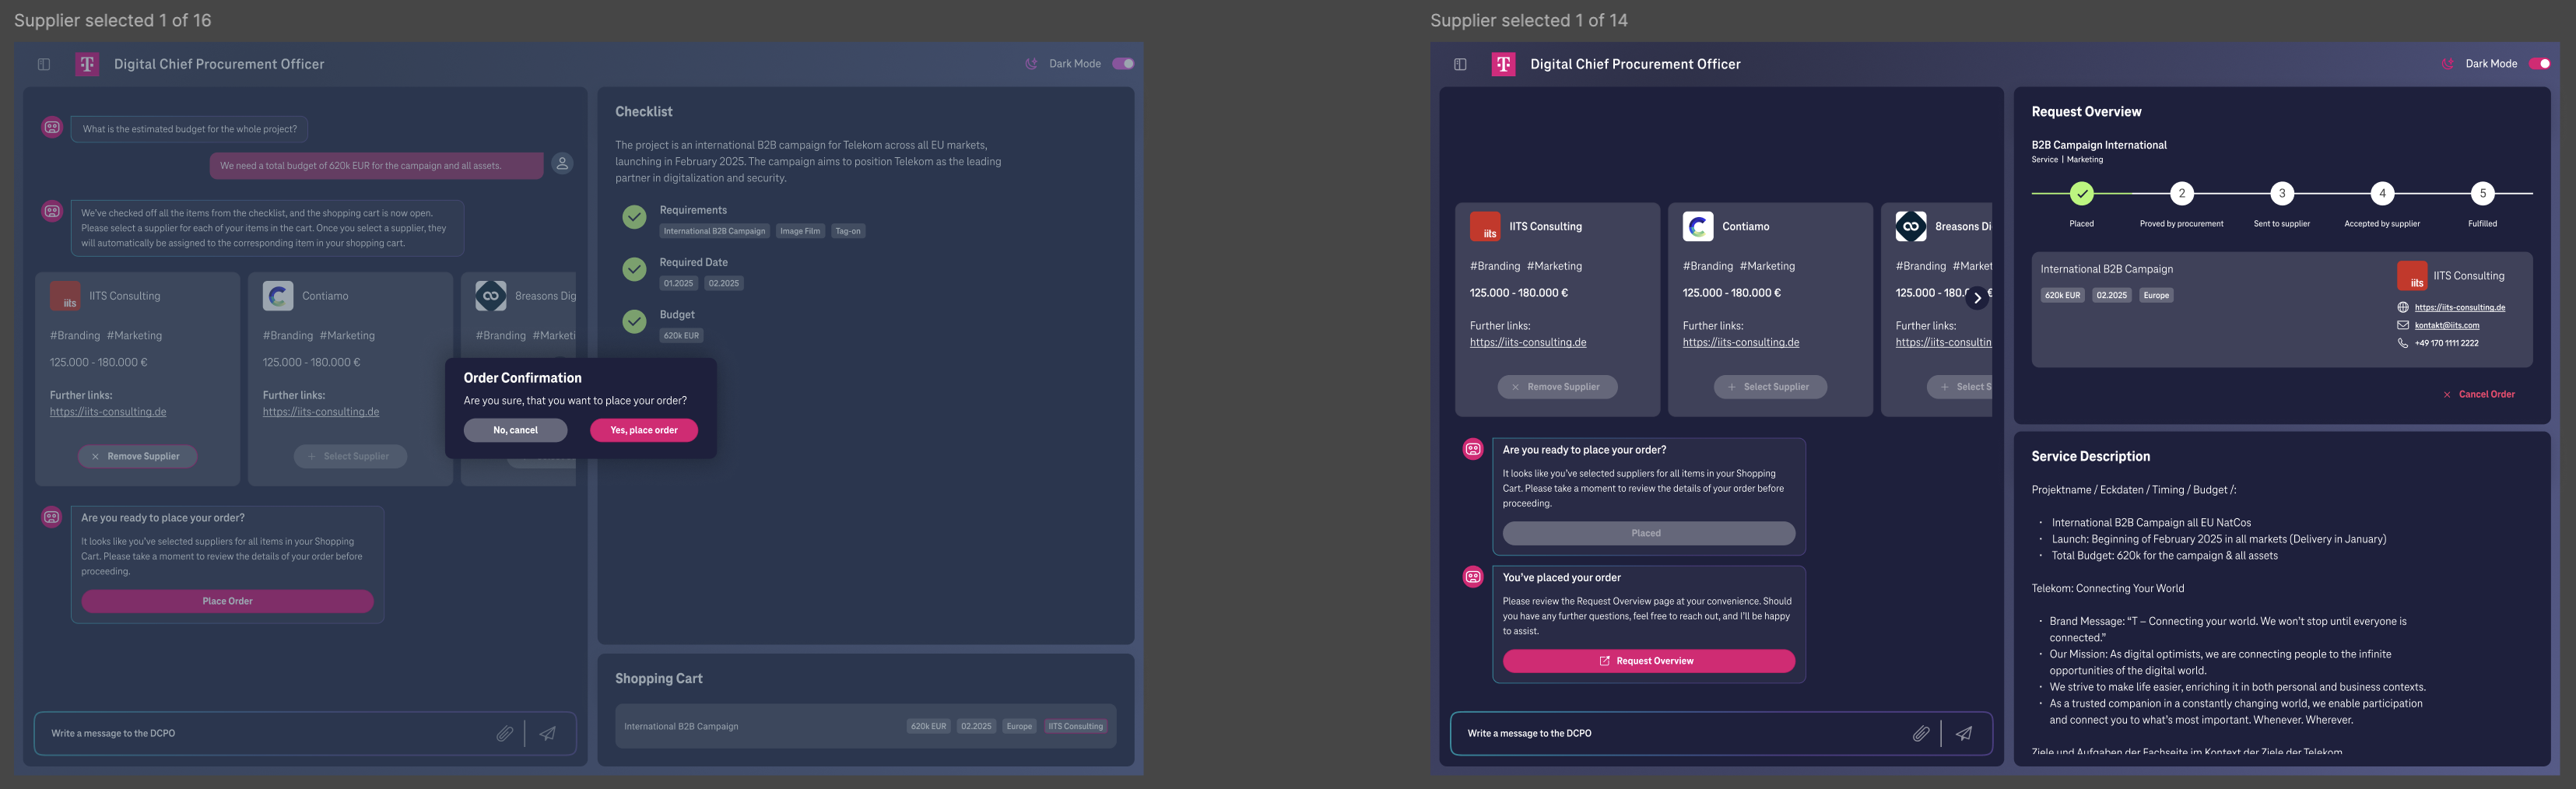
\includegraphics[width=1\textwidth]{abbildungen/RE/Figma/Figma_Screens-Darkmode}
\end{figure}
\footnotetext{Own illustration}

Once the Figma designs were validated, the project moved to the development of functional builds using Vue. These builds
marked the first instance of the system in a live environment, where the chatbot could be tested in real-time against
actual user inputs. The Vue builds, examples shown in figure
%TODO Ref for Vue Figures
provided the opportunity to verify that the system met the documented requirements in
practice, with users engaging directly with the chatbot interface to simulate procurement scenarios. During these tests,
it became evident whether the chatbot’s decision-making processes were functioning as expected and whether its
performance, particularly in searching supplier catalogs and handling user requests, met the defined non-functional
requirements. The feedback gathered during this phase led to further adjustments, with particular focus on optimizing
the chatbot’s responsiveness and ensuring the smooth integration of supplier data into the system’s workflow.

%TODO Add Vue Screens

The culmination of the Requirement Elicitation phase was the consolidation of all gathered requirements into a
structured document that served as the definitive guide for the project’s development. This document captured the full
scope of the system’s functional and non-functional needs, including the precise behavior of the chatbot when
interacting with users, the expected performance standards, and the overall user experience considerations. This
requirements document evolved alongside the project, incorporating feedback from stakeholders at each stage—from the
Miro mockups to the Figma prototypes and finally the Vue builds—ensuring that the requirements were fully traceable
throughout the entire development process. The result of this phase was a clear, comprehensive set of requirements that
not only reflected the needs of the users but also aligned with the technical constraints and objectives of the system,
providing a solid foundation for the subsequent stages of development.

\subsection{Requirement Analysis and Negotiation}\label{subsec:requirement-analysis-and-negotiation}

The Requirement Analysis and Negotiation phase focused on refining the gathered requirements and resolving any conflicts
or ambiguities that arose during the elicitation phase. This stage was essential for ensuring that the system would meet
both the technical constraints and the diverse needs of the various stakeholders involved in the project. The process of
analysis and negotiation was conducted primarily through regular weekly meetings with stakeholders and bi-weekly
sessions with senior management, ensuring that the project stayed aligned with both operational expectations and
strategic objectives.

The weekly meetings with stakeholders formed the backbone of the Requirement Analysis process. These sessions, which
brought together representatives from the procurement teams, technical staff, and other key user groups, provided a
structured environment for ongoing discussions about the system’s requirements. During these meetings, the feedback
gathered from the prototyping phases was reviewed in detail, with particular attention given to how the system’s
functionalities were evolving in response to the requirements initially defined in the workshops.

A key aspect of these weekly sessions was the continuous prioritization of requirements. The stakeholders provided input
on which features needed to be refined or developed first, helping the \acs{PO} maintain focus on core functionalities,
such as the chatbot's ability to interpret and act on user requests. These discussions also enabled the \acs{PO} to identify
any gaps in the requirements or areas where further clarification was needed, ensuring that the chatbot’s functionality
would align with the intended procurement processes.

In addition to prioritization, the weekly meetings were also used to resolve conflicts between competing requirements.
As different stakeholders had varying expectations of how the chatbot should function, these sessions served as a forum
for negotiation. For example, there were often trade-offs between modern design and user accessibility, or between
performance and cost. By bringing these issues to the forefront in a collaborative setting, the \acs{PO} was able to reach
consensus on the best approach to take. These discussions were particularly valuable in clarifying the chatbot’s core
functionalities, such as determining the appropriate level of detail the chatbot should provide when responding to user
queries and how it should handle requests that were not well-defined.

Through these weekly discussions, the \acs{PO} was able to continuously refine the system’s requirements, ensuring that
they remained both feasible and aligned with the overall project goals. As new insights emerged, they were integrated
into the requirements document, ensuring that the evolving needs of the stakeholders were captured and could be tracked
throughout the development process.

In parallel with the weekly stakeholder sessions, bi-weekly meetings with senior management were held to ensure that the
project remained aligned with the broader strategic objectives of the organization. These meetings provided a
higher-level perspective on the system’s development, focusing on ensuring that the chatbot’s functionalities would not
only meet the immediate operational needs but also support the company’s long-term goals for procurement efficiency and
digital transformation.

The bi-weekly management meetings were critical in securing approvals for key decisions made during the Requirement
Analysis phase. For instance, as the system’s development progressed and the trade-offs between performance and cost
became more apparent, it was essential to have senior management’s input to determine the acceptable levels of
investment in system performance. These meetings also provided an opportunity to discuss the prioritization of
high-impact features, ensuring that the project remained focused on delivering value in line with the company’s
strategic initiatives.

One important aspect of the bi-weekly management meetings was the focus on risk mitigation. As potential risks were
identified during the stakeholder meetings, such as delays in catalog integration or challenges related to system
scalability, these issues were brought to the attention of senior management. This allowed the \acs{PO} to make
informed decisions about how to allocate resources and manage risks effectively, ensuring that the system development
remained on track and that any potential bottlenecks could be addressed early.

The management meetings also served as a platform to reflect the progress made in the weekly stakeholder sessions. By
reviewing the decisions made and the requirements refined during those discussions, senior management was able to
provide feedback and ensure that the system’s development remained consistent with the organization’s vision. This
continuous feedback loop between the weekly stakeholder sessions and the bi-weekly management reviews ensured that the
system’s development remained agile and responsive to both operational and strategic needs.

The iterative nature of the Requirement Analysis and Negotiation phase allowed for continuous refinement of the
chatbot’s requirements. The weekly stakeholder meetings provided detailed input on the system’s functionality and
performance, while the bi-weekly management meetings ensured that these decisions aligned with the organization’s
broader goals. Throughout this phase, the requirements document was continuously updated, reflecting the outcomes of
each discussion and ensuring that every decision was documented and traceable.

\subsection{Requirement Validation}\label{subsec:requirement-validation}

The Requirement Validation phase was critical in ensuring that the requirements gathered and refined in previous phases
were accurate, complete, and feasible. The goal was to verify that the functional and non-functional needs of the system
were well understood and aligned with stakeholder expectations. This phase relied on interactive tools such as Figma
prototypes to visualize and simulate the chatbot’s core functionalities. In addition, initial backend conversations were
tested during this phase to verify key technical aspects of the chatbot’s processing logic.

The Figma prototypes played a crucial role in validating the system’s design and behavior. These prototypes allowed
stakeholders to interact with a detailed and high-fidelity representation of how the chatbot would operate in practice.
They offered a clear view of the user interface, navigation, and interaction flows, simulating the chatbot’s procurement
process without requiring full backend integration or live data.

Stakeholders were invited to explore these prototypes, providing feedback on whether the user experience and
functionality met the documented requirements. The prototypes simulated key features such as the chatbot’s response to
user inputs, search functionality within supplier catalogs, and the overall flow from request initiation to the
presentation of recommendations. This validation helped identify any areas where the chatbot’s design needed to be
adjusted to better meet business objectives. Based on stakeholder feedback, improvements were made to enhance usability
and ensure the chatbot’s interaction with users was intuitive and aligned with the intended procurement processes.

%TODO Wie wurde das Backend getestet
In addition to validating the user interface through Figma prototypes, early backend conversations were also validated
in this phase. This validation focused on ensuring that the backend could interpret user input and return appropriate
responses, even though the system was not yet fully integrated or using live data. By simulating conversations between
the chatbot and users, the \acs{PO} was able to validate that the backend logic was functioning correctly and that the
chatbot could handle simple dialogues.

These initial backend tests provided valuable insights into how the chatbot’s \acs{NLP} would work in practice, allowing
the \acs{PO} to refine the backend’s ability to interpret requests and provide relevant responses. Testing these
conversations during the validation phase ensured that both the frontend prototypes and backend logic were progressing
in alignment with the documented requirements.

Throughout the Requirement Validation phase, regular review sessions were conducted with stakeholders to gather ongoing
feedback. These sessions were essential for ensuring that the evolving prototypes and backend functionalities were
meeting expectations. The interactive nature of these reviews allowed stakeholders to provide detailed feedback on the
chatbot’s behavior, leading to continuous refinements of both the design and backend logic.

Key areas of focus during these reviews included validating the accuracy of the chatbot’s responses, ensuring smooth
navigation, and confirming that the user interface was intuitive. The feedback provided by stakeholders was incorporated
into subsequent iterations of the prototypes and backend logic, ensuring that the system continued to evolve in line
with the project’s goals.

After successfully validating the requirements through both the Figma prototypes and early backend tests, the \acs{PO}
was ready to move into the actual development phase. The transition marked the end of the Requirement Validation phase,
signaling that the requirements had been thoroughly vetted and were ready for implementation. With the core
functionalities validated and feedback incorporated, the development of the full prototype, including both the backend
and frontend systems, began using test data.

\subsection{Requirement Management}\label{subsec:requirement-management}

The Requirement Management phase focused on maintaining control over the evolving requirements throughout the project.
As new insights emerged from stakeholder feedback and validation sessions, it was essential to manage changes
systematically to ensure that all modifications were properly documented and traceable. A structured approach was
adopted to track every change in the requirements, ensuring that the \acs{PO} and stakeholders remained aligned on any
updates or shifts in priorities. This process helped avoid scope creep and ensured that only approved changes were
implemented, safeguarding the integrity of the original project objectives.

Regular reviews of the requirements document were conducted to reflect the evolving nature of the project, particularly
as feedback from the validation phase led to refinements in the system’s functionality. By maintaining up-to-date
records of all changes, the \acs{PO} was able to ensure consistency between the original requirements and the final
deliverables. This approach ensured that any changes were justified, reviewed, and incorporated without disrupting the
overall project flow, providing a robust framework for managing the dynamic aspects of the chatbot’s development. The
complete set of these finalized documents can be found in \ref{subsec:filled-out-requirement-documents} for further
reference.
